% Options for packages loaded elsewhere
\PassOptionsToPackage{unicode}{hyperref}
\PassOptionsToPackage{hyphens}{url}
\PassOptionsToPackage{dvipsnames,svgnames,x11names}{xcolor}
%
\documentclass[
  a4paper,
  DIV=11,
  numbers=noendperiod]{scrartcl}

\usepackage{amsmath,amssymb}
\usepackage{lmodern}
\usepackage{iftex}
\ifPDFTeX
  \usepackage[T1]{fontenc}
  \usepackage[utf8]{inputenc}
  \usepackage{textcomp} % provide euro and other symbols
\else % if luatex or xetex
  \usepackage{unicode-math}
  \defaultfontfeatures{Scale=MatchLowercase}
  \defaultfontfeatures[\rmfamily]{Ligatures=TeX,Scale=1}
\fi
% Use upquote if available, for straight quotes in verbatim environments
\IfFileExists{upquote.sty}{\usepackage{upquote}}{}
\IfFileExists{microtype.sty}{% use microtype if available
  \usepackage[]{microtype}
  \UseMicrotypeSet[protrusion]{basicmath} % disable protrusion for tt fonts
}{}
\makeatletter
\@ifundefined{KOMAClassName}{% if non-KOMA class
  \IfFileExists{parskip.sty}{%
    \usepackage{parskip}
  }{% else
    \setlength{\parindent}{0pt}
    \setlength{\parskip}{6pt plus 2pt minus 1pt}}
}{% if KOMA class
  \KOMAoptions{parskip=half}}
\makeatother
\usepackage{xcolor}
\usepackage[top=30mm,left=15mm,right = 15mm,heightrounded]{geometry}
\setlength{\emergencystretch}{3em} % prevent overfull lines
\setcounter{secnumdepth}{5}
% Make \paragraph and \subparagraph free-standing
\ifx\paragraph\undefined\else
  \let\oldparagraph\paragraph
  \renewcommand{\paragraph}[1]{\oldparagraph{#1}\mbox{}}
\fi
\ifx\subparagraph\undefined\else
  \let\oldsubparagraph\subparagraph
  \renewcommand{\subparagraph}[1]{\oldsubparagraph{#1}\mbox{}}
\fi

\usepackage{color}
\usepackage{fancyvrb}
\newcommand{\VerbBar}{|}
\newcommand{\VERB}{\Verb[commandchars=\\\{\}]}
\DefineVerbatimEnvironment{Highlighting}{Verbatim}{commandchars=\\\{\}}
% Add ',fontsize=\small' for more characters per line
\usepackage{framed}
\definecolor{shadecolor}{RGB}{241,243,245}
\newenvironment{Shaded}{\begin{snugshade}}{\end{snugshade}}
\newcommand{\AlertTok}[1]{\textcolor[rgb]{0.68,0.00,0.00}{#1}}
\newcommand{\AnnotationTok}[1]{\textcolor[rgb]{0.37,0.37,0.37}{#1}}
\newcommand{\AttributeTok}[1]{\textcolor[rgb]{0.40,0.45,0.13}{#1}}
\newcommand{\BaseNTok}[1]{\textcolor[rgb]{0.68,0.00,0.00}{#1}}
\newcommand{\BuiltInTok}[1]{\textcolor[rgb]{0.00,0.23,0.31}{#1}}
\newcommand{\CharTok}[1]{\textcolor[rgb]{0.13,0.47,0.30}{#1}}
\newcommand{\CommentTok}[1]{\textcolor[rgb]{0.37,0.37,0.37}{#1}}
\newcommand{\CommentVarTok}[1]{\textcolor[rgb]{0.37,0.37,0.37}{\textit{#1}}}
\newcommand{\ConstantTok}[1]{\textcolor[rgb]{0.56,0.35,0.01}{#1}}
\newcommand{\ControlFlowTok}[1]{\textcolor[rgb]{0.00,0.23,0.31}{#1}}
\newcommand{\DataTypeTok}[1]{\textcolor[rgb]{0.68,0.00,0.00}{#1}}
\newcommand{\DecValTok}[1]{\textcolor[rgb]{0.68,0.00,0.00}{#1}}
\newcommand{\DocumentationTok}[1]{\textcolor[rgb]{0.37,0.37,0.37}{\textit{#1}}}
\newcommand{\ErrorTok}[1]{\textcolor[rgb]{0.68,0.00,0.00}{#1}}
\newcommand{\ExtensionTok}[1]{\textcolor[rgb]{0.00,0.23,0.31}{#1}}
\newcommand{\FloatTok}[1]{\textcolor[rgb]{0.68,0.00,0.00}{#1}}
\newcommand{\FunctionTok}[1]{\textcolor[rgb]{0.28,0.35,0.67}{#1}}
\newcommand{\ImportTok}[1]{\textcolor[rgb]{0.00,0.46,0.62}{#1}}
\newcommand{\InformationTok}[1]{\textcolor[rgb]{0.37,0.37,0.37}{#1}}
\newcommand{\KeywordTok}[1]{\textcolor[rgb]{0.00,0.23,0.31}{#1}}
\newcommand{\NormalTok}[1]{\textcolor[rgb]{0.00,0.23,0.31}{#1}}
\newcommand{\OperatorTok}[1]{\textcolor[rgb]{0.37,0.37,0.37}{#1}}
\newcommand{\OtherTok}[1]{\textcolor[rgb]{0.00,0.23,0.31}{#1}}
\newcommand{\PreprocessorTok}[1]{\textcolor[rgb]{0.68,0.00,0.00}{#1}}
\newcommand{\RegionMarkerTok}[1]{\textcolor[rgb]{0.00,0.23,0.31}{#1}}
\newcommand{\SpecialCharTok}[1]{\textcolor[rgb]{0.37,0.37,0.37}{#1}}
\newcommand{\SpecialStringTok}[1]{\textcolor[rgb]{0.13,0.47,0.30}{#1}}
\newcommand{\StringTok}[1]{\textcolor[rgb]{0.13,0.47,0.30}{#1}}
\newcommand{\VariableTok}[1]{\textcolor[rgb]{0.07,0.07,0.07}{#1}}
\newcommand{\VerbatimStringTok}[1]{\textcolor[rgb]{0.13,0.47,0.30}{#1}}
\newcommand{\WarningTok}[1]{\textcolor[rgb]{0.37,0.37,0.37}{\textit{#1}}}

\providecommand{\tightlist}{%
  \setlength{\itemsep}{0pt}\setlength{\parskip}{0pt}}\usepackage{longtable,booktabs,array}
\usepackage{calc} % for calculating minipage widths
% Correct order of tables after \paragraph or \subparagraph
\usepackage{etoolbox}
\makeatletter
\patchcmd\longtable{\par}{\if@noskipsec\mbox{}\fi\par}{}{}
\makeatother
% Allow footnotes in longtable head/foot
\IfFileExists{footnotehyper.sty}{\usepackage{footnotehyper}}{\usepackage{footnote}}
\makesavenoteenv{longtable}
\usepackage{graphicx}
\makeatletter
\def\maxwidth{\ifdim\Gin@nat@width>\linewidth\linewidth\else\Gin@nat@width\fi}
\def\maxheight{\ifdim\Gin@nat@height>\textheight\textheight\else\Gin@nat@height\fi}
\makeatother
% Scale images if necessary, so that they will not overflow the page
% margins by default, and it is still possible to overwrite the defaults
% using explicit options in \includegraphics[width, height, ...]{}
\setkeys{Gin}{width=\maxwidth,height=\maxheight,keepaspectratio}
% Set default figure placement to htbp
\makeatletter
\def\fps@figure{htbp}
\makeatother

\KOMAoption{captions}{tableheading}
\makeatletter
\makeatother
\makeatletter
\makeatother
\makeatletter
\@ifpackageloaded{caption}{}{\usepackage{caption}}
\AtBeginDocument{%
\ifdefined\contentsname
  \renewcommand*\contentsname{Table of contents}
\else
  \newcommand\contentsname{Table of contents}
\fi
\ifdefined\listfigurename
  \renewcommand*\listfigurename{List of Figures}
\else
  \newcommand\listfigurename{List of Figures}
\fi
\ifdefined\listtablename
  \renewcommand*\listtablename{List of Tables}
\else
  \newcommand\listtablename{List of Tables}
\fi
\ifdefined\figurename
  \renewcommand*\figurename{Figure}
\else
  \newcommand\figurename{Figure}
\fi
\ifdefined\tablename
  \renewcommand*\tablename{Table}
\else
  \newcommand\tablename{Table}
\fi
}
\@ifpackageloaded{float}{}{\usepackage{float}}
\floatstyle{ruled}
\@ifundefined{c@chapter}{\newfloat{codelisting}{h}{lop}}{\newfloat{codelisting}{h}{lop}[chapter]}
\floatname{codelisting}{Listing}
\newcommand*\listoflistings{\listof{codelisting}{List of Listings}}
\makeatother
\makeatletter
\@ifpackageloaded{caption}{}{\usepackage{caption}}
\@ifpackageloaded{subcaption}{}{\usepackage{subcaption}}
\makeatother
\makeatletter
\@ifpackageloaded{tcolorbox}{}{\usepackage[many]{tcolorbox}}
\makeatother
\makeatletter
\@ifundefined{shadecolor}{\definecolor{shadecolor}{rgb}{.97, .97, .97}}
\makeatother
\makeatletter
\makeatother
\ifLuaTeX
  \usepackage{selnolig}  % disable illegal ligatures
\fi
\IfFileExists{bookmark.sty}{\usepackage{bookmark}}{\usepackage{hyperref}}
\IfFileExists{xurl.sty}{\usepackage{xurl}}{} % add URL line breaks if available
\urlstyle{same} % disable monospaced font for URLs
\hypersetup{
  pdftitle={Stats},
  colorlinks=true,
  linkcolor={blue},
  filecolor={Maroon},
  citecolor={Blue},
  urlcolor={Blue},
  pdfcreator={LaTeX via pandoc}}

\title{Stats}
\author{}
\date{}

\begin{document}
\maketitle
\ifdefined\Shaded\renewenvironment{Shaded}{\begin{tcolorbox}[borderline west={3pt}{0pt}{shadecolor}, boxrule=0pt, sharp corners, interior hidden, frame hidden, breakable, enhanced]}{\end{tcolorbox}}\fi

\renewcommand*\contentsname{Table of contents}
{
\hypersetup{linkcolor=}
\setcounter{tocdepth}{3}
\tableofcontents
}
\begin{Shaded}
\begin{Highlighting}[]
\FunctionTok{library}\NormalTok{(tidyr)}
\FunctionTok{library}\NormalTok{(tidyverse)}
\end{Highlighting}
\end{Shaded}

\begin{verbatim}
-- Attaching packages --------------------------------------- tidyverse 1.3.2 --
v ggplot2 3.3.6      v dplyr   1.0.10
v tibble  3.1.8      v stringr 1.4.1 
v readr   2.1.3      v forcats 0.5.2 
v purrr   0.3.4      
-- Conflicts ------------------------------------------ tidyverse_conflicts() --
x dplyr::filter() masks stats::filter()
x dplyr::lag()    masks stats::lag()
\end{verbatim}

\begin{Shaded}
\begin{Highlighting}[]
\FunctionTok{library}\NormalTok{(ggplot2)}
\FunctionTok{library}\NormalTok{(GGally)}
\end{Highlighting}
\end{Shaded}

\begin{verbatim}
Registered S3 method overwritten by 'GGally':
  method from   
  +.gg   ggplot2
\end{verbatim}

\begin{Shaded}
\begin{Highlighting}[]
\NormalTok{ozone }\OtherTok{=} \FunctionTok{read\_csv}\NormalTok{(}\StringTok{"ozone.csv"}\NormalTok{)}
\end{Highlighting}
\end{Shaded}

\begin{verbatim}
Rows: 111 Columns: 4
-- Column specification --------------------------------------------------------
Delimiter: ","
dbl (4): radiation, temperature, wind, ozone

i Use `spec()` to retrieve the full column specification for this data.
i Specify the column types or set `show_col_types = FALSE` to quiet this message.
\end{verbatim}

\#\#Question 1 a)

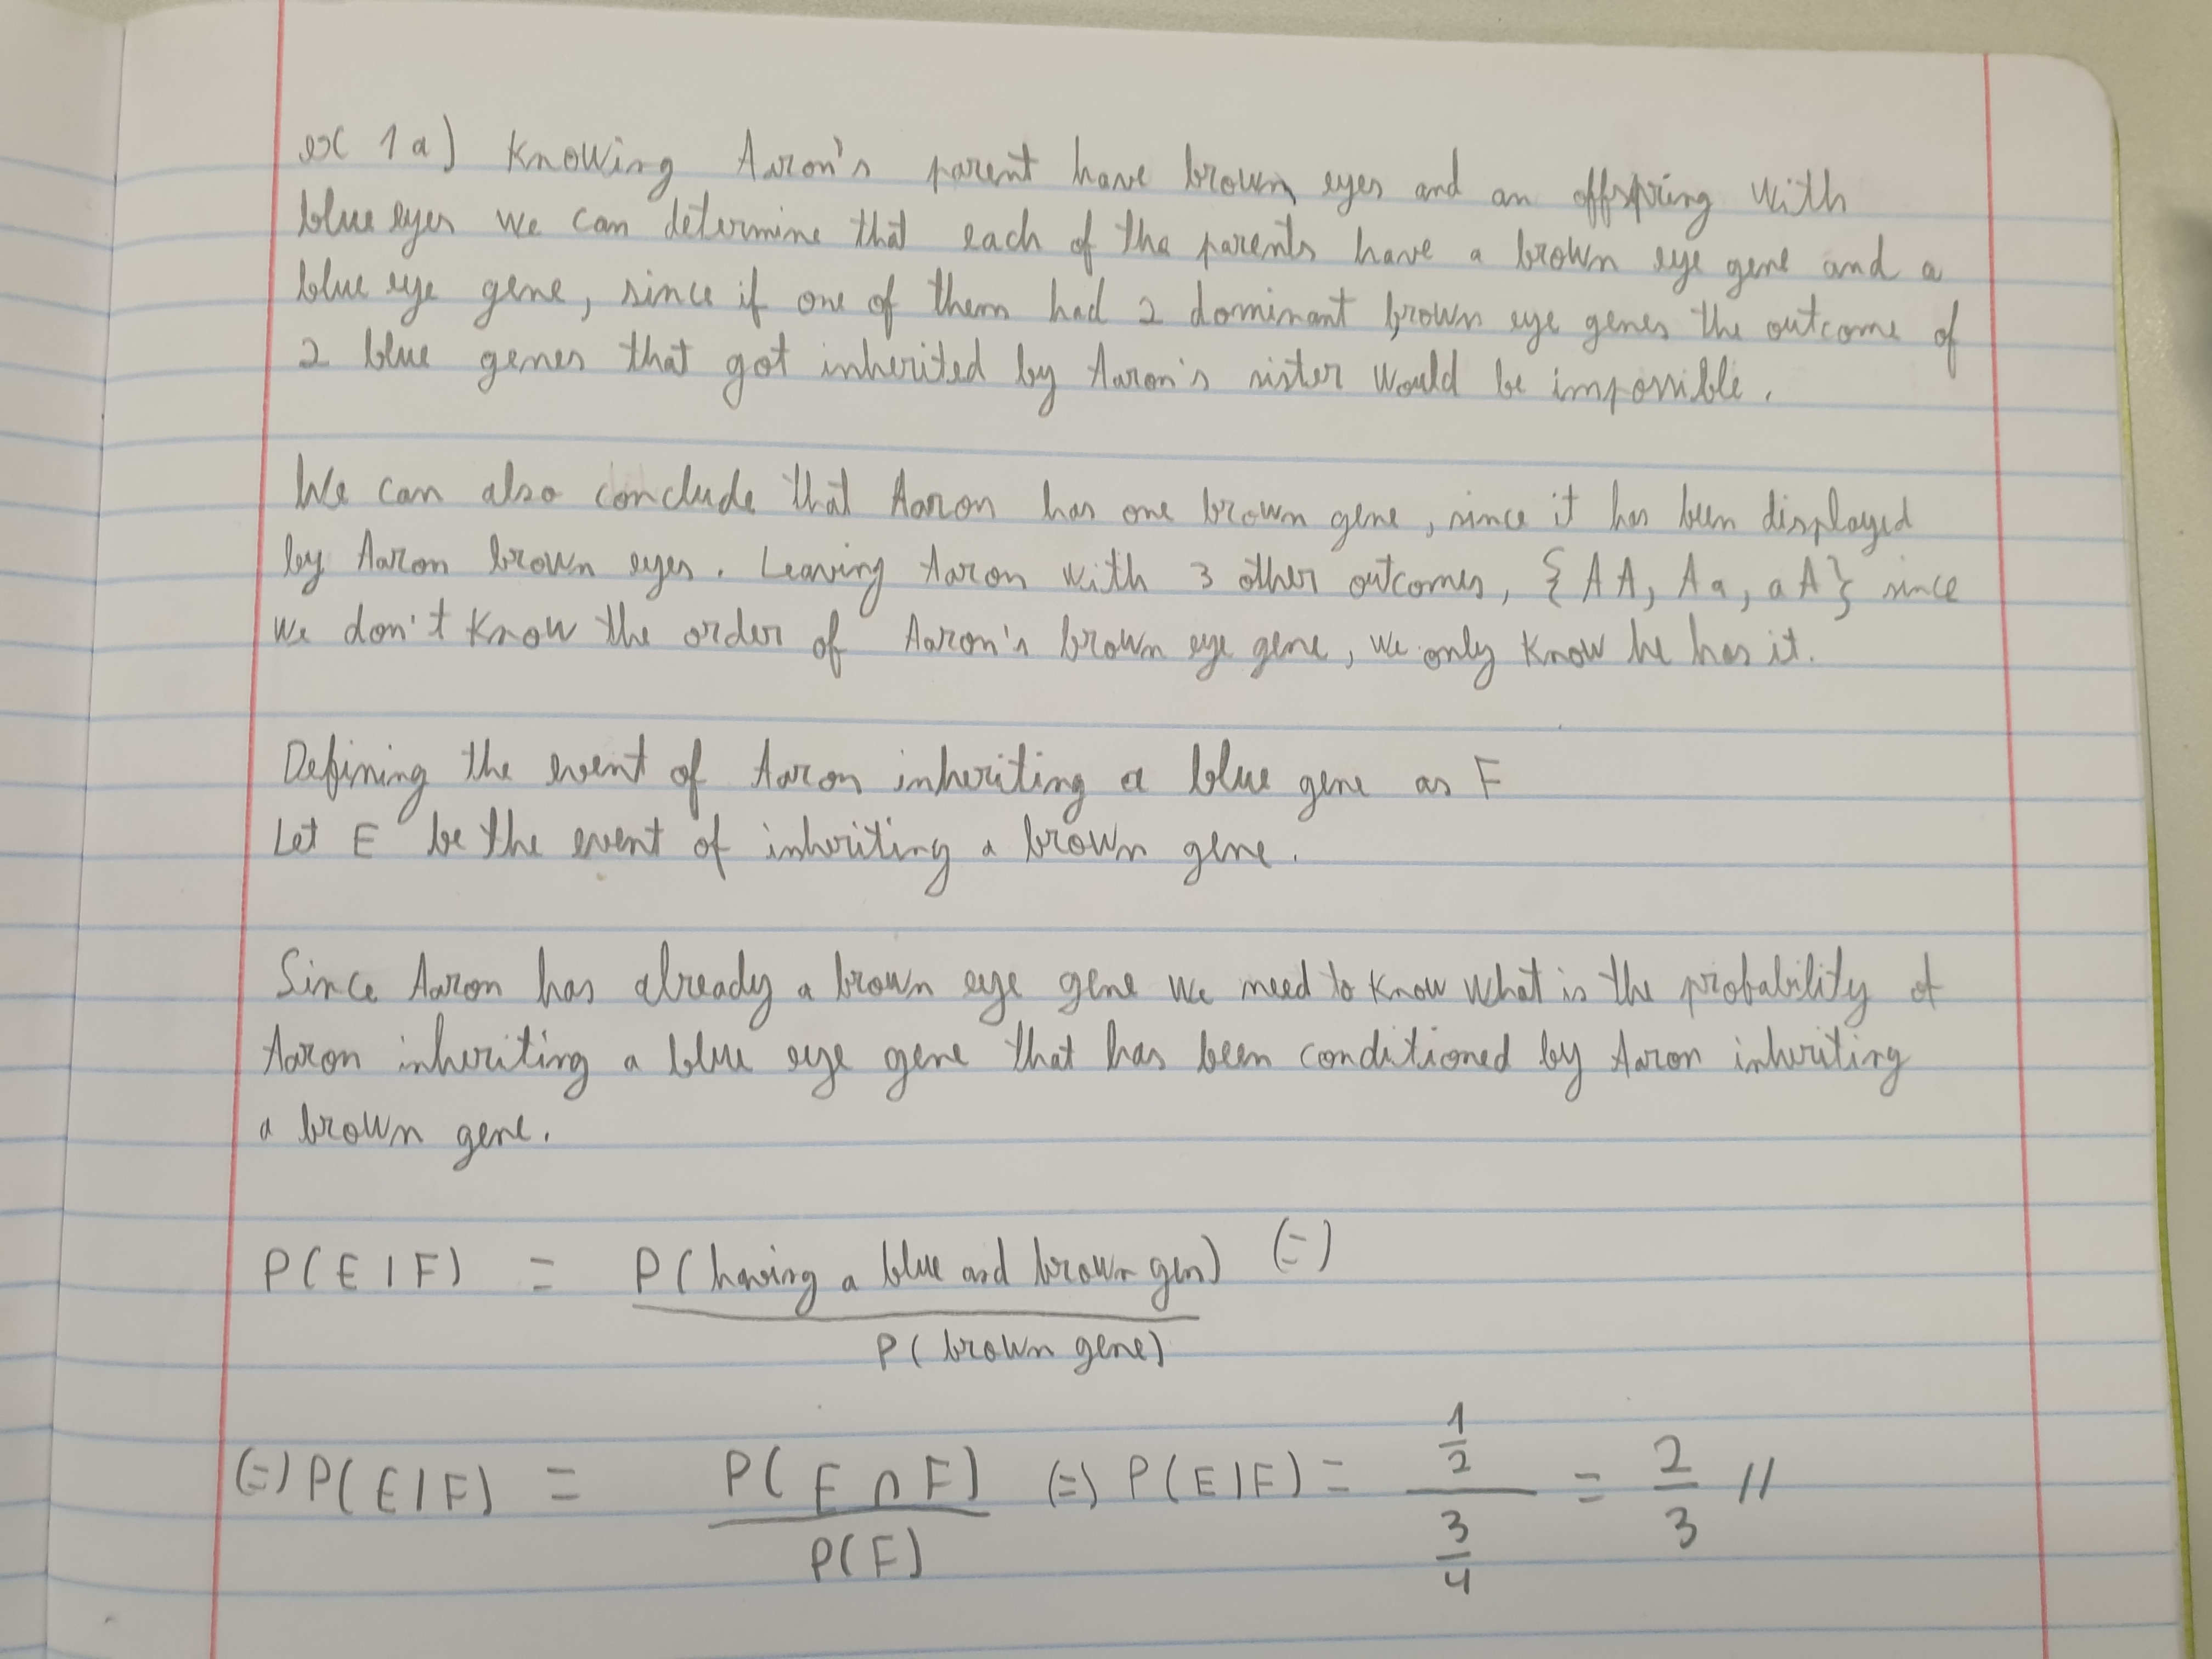
\includegraphics{1a.pdf}.jpg)

\#\#Question 1 b)

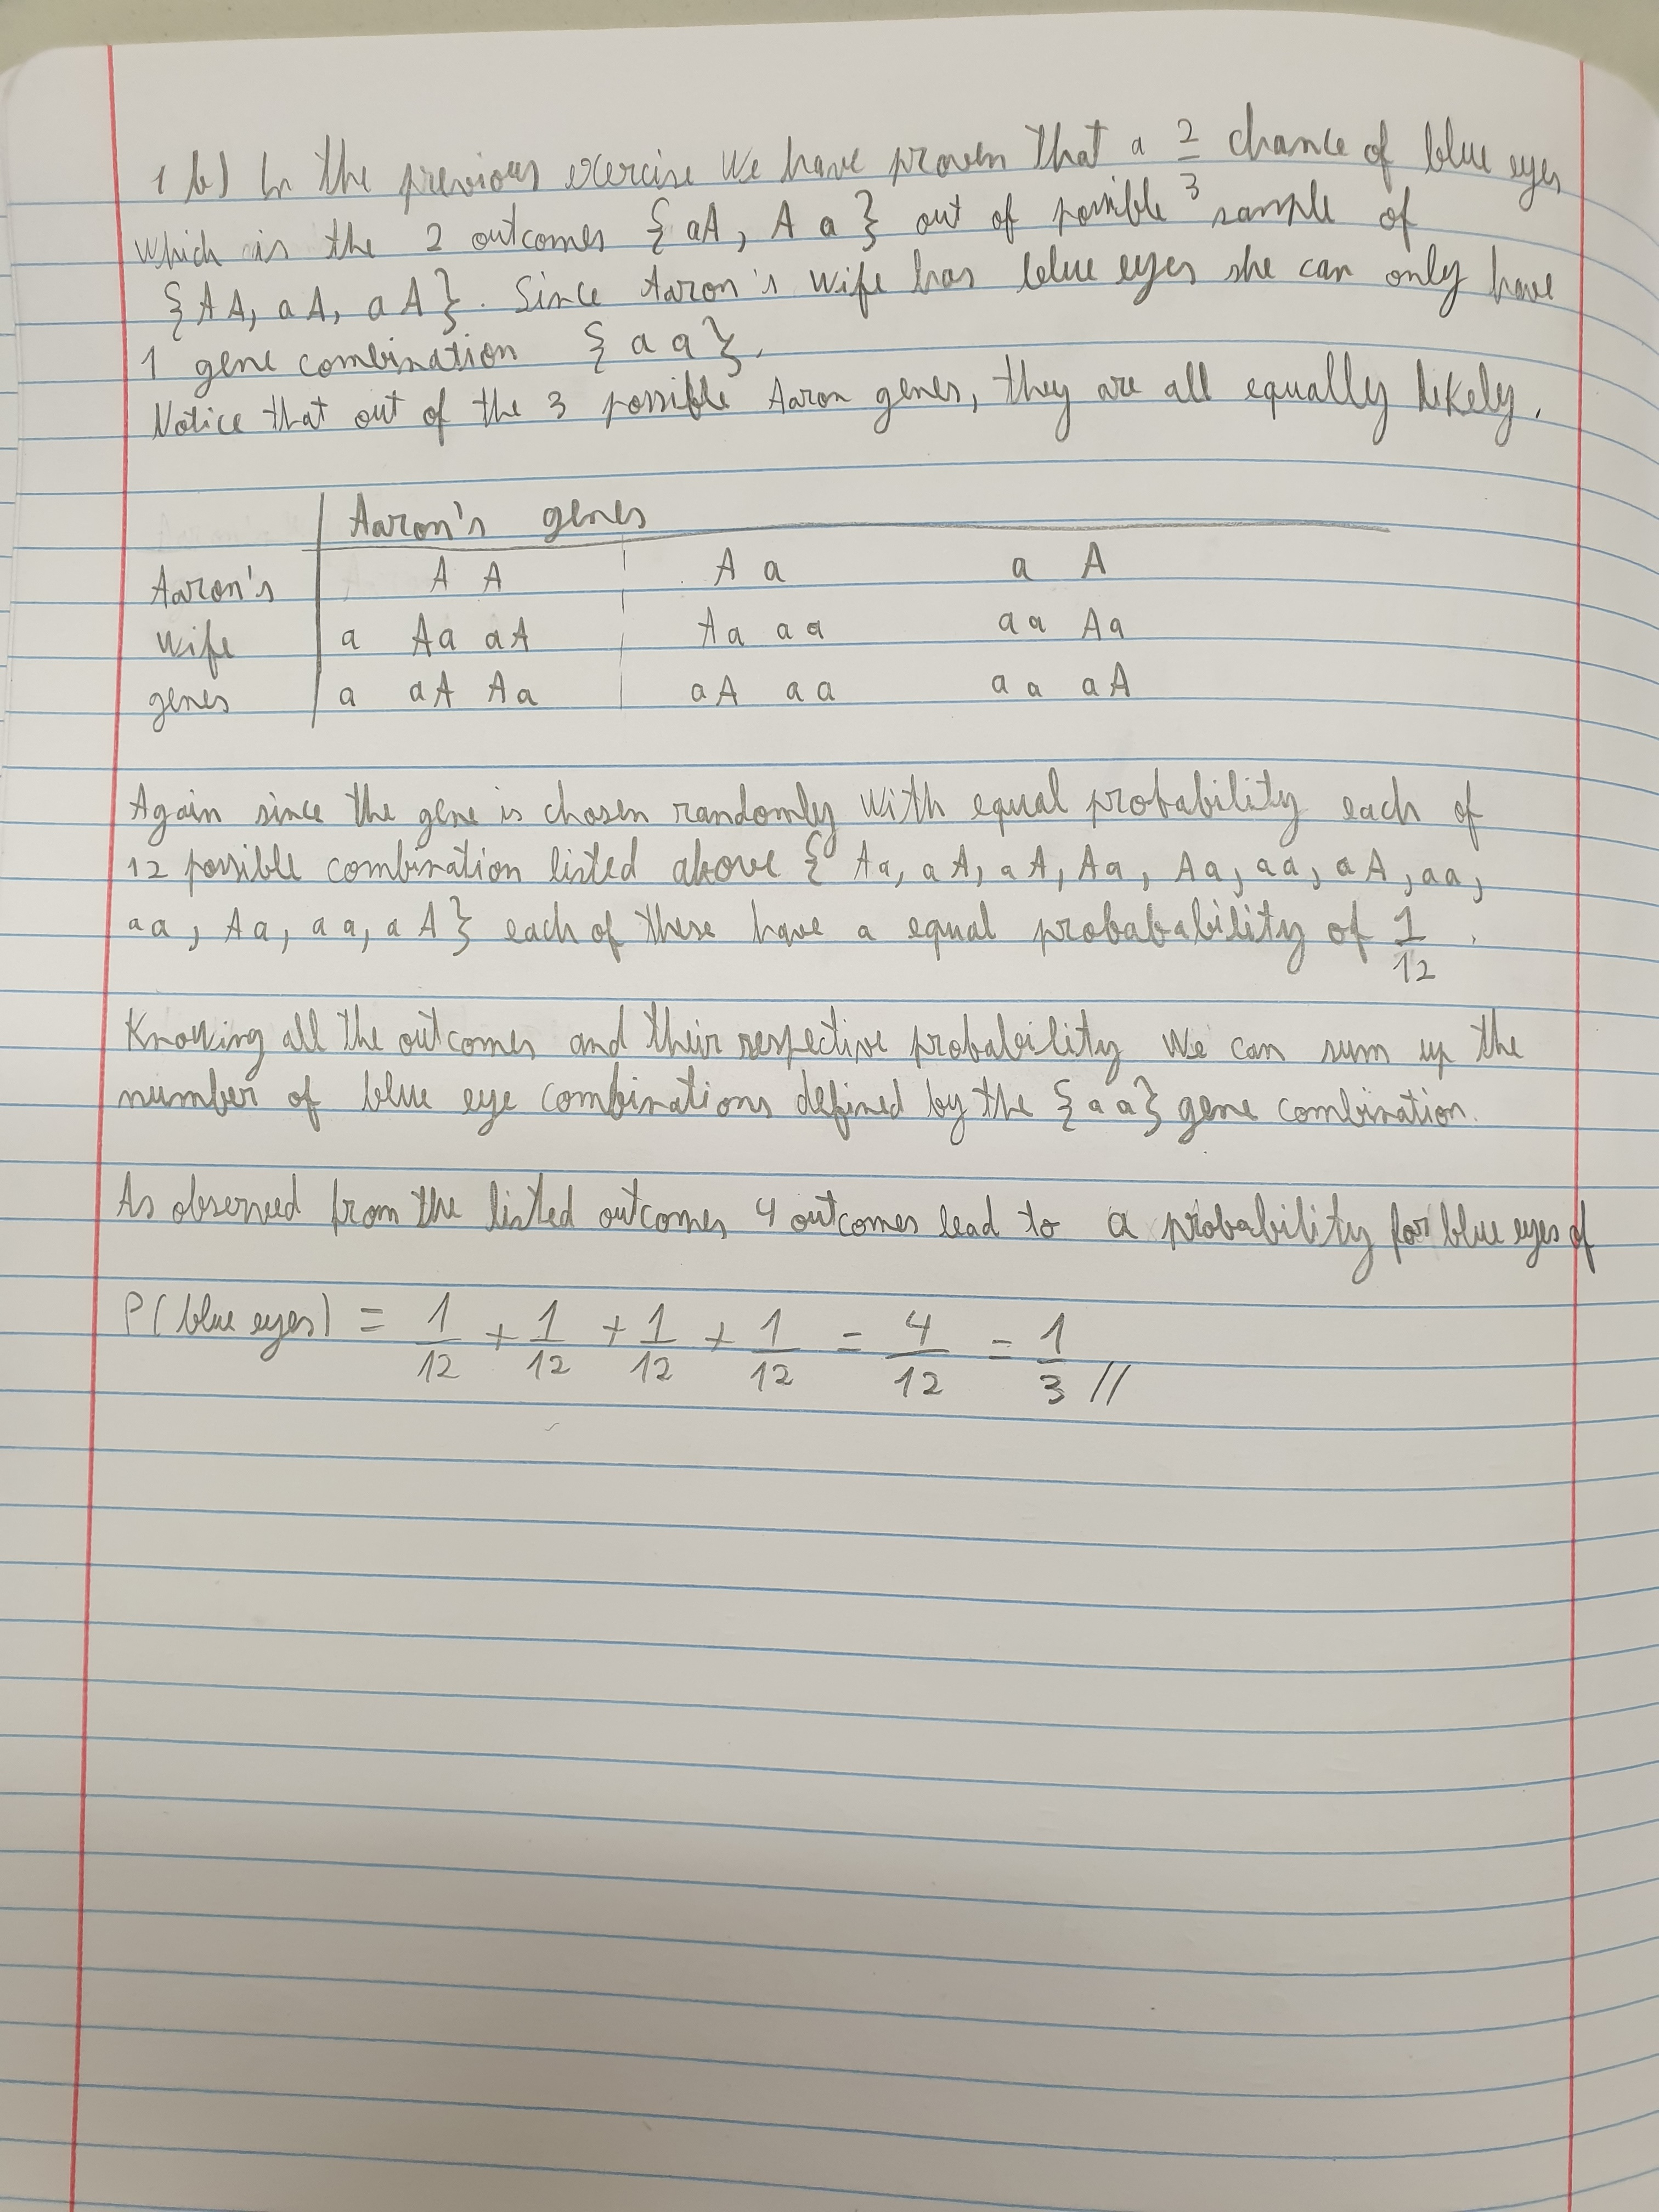
\includegraphics{1b.pdf}.jpg)

\#\#Question 1 c)

Part 1 of exercise 1 c) \includegraphics{1c.pdf}-part1.jpg)

Part 2 of exercise 1 c) \includegraphics{1c.pdf}-part2.jpg)

\#\#Question 2 a)

Part 1 of exercise 2 a) \includegraphics{2a.pdf}-part1.jpg)

Part 2 of exercise 2 a) \includegraphics{2a.pdf}-part2.jpg)

\#\#question 2 C)

\begin{Shaded}
\begin{Highlighting}[]
\CommentTok{\# set.seed(26041999)}

\NormalTok{candidateBWins }\OtherTok{=} \DecValTok{0}

\DocumentationTok{\#\# Here we set the number of times we will estimate}
\NormalTok{largeNumberOfExtimations }\OtherTok{=} \FloatTok{1e+06}

\ControlFlowTok{for}\NormalTok{ (i }\ControlFlowTok{in} \DecValTok{1}\SpecialCharTok{:}\NormalTok{largeNumberOfExtimations) \{}

\NormalTok{    candidateB }\OtherTok{=} \DecValTok{175}  \DocumentationTok{\#\# candidate B initial votes/support}
\NormalTok{    candidateM }\OtherTok{=} \DecValTok{184}  \DocumentationTok{\#\# candidate M initial votes/support}

    \DocumentationTok{\#\# increment for each day from the initial day to the final day,}
    \DocumentationTok{\#\# the 14th}
    \ControlFlowTok{for}\NormalTok{ (i }\ControlFlowTok{in} \DecValTok{1}\SpecialCharTok{:}\DecValTok{14}\NormalTok{) \{}

        \DocumentationTok{\#\# will be used to hold the new value of votes that continue to}
        \DocumentationTok{\#\# support the same candidate}
\NormalTok{        candidateBAuxCalc }\OtherTok{=} \DecValTok{0}
\NormalTok{        candidateMAuxCalc }\OtherTok{=} \DecValTok{0}

        \DocumentationTok{\#\# here we will estimate how many candidates still support the}
        \DocumentationTok{\#\# same candidate by generating a vector where 1 means they}
        \DocumentationTok{\#\# still support the same candidate after the end of each day}
        \DocumentationTok{\#\# the 0 represent them changing the support and vote from one}
        \DocumentationTok{\#\# candidate to another}
\NormalTok{        candidateBAuxCalc }\OtherTok{=} \FunctionTok{sum}\NormalTok{(}\FunctionTok{sample}\NormalTok{(}\FunctionTok{c}\NormalTok{(}\DecValTok{1}\NormalTok{, }\DecValTok{0}\NormalTok{), candidateB, }\AttributeTok{replace =} \ConstantTok{TRUE}\NormalTok{,}
            \AttributeTok{prob =} \FunctionTok{c}\NormalTok{(}\FloatTok{0.996}\NormalTok{, }\FloatTok{0.004}\NormalTok{)))}
\NormalTok{        candidateMAuxCalc }\OtherTok{=} \FunctionTok{sum}\NormalTok{(}\FunctionTok{sample}\NormalTok{(}\FunctionTok{c}\NormalTok{(}\DecValTok{1}\NormalTok{, }\DecValTok{0}\NormalTok{), candidateM, }\AttributeTok{replace =} \ConstantTok{TRUE}\NormalTok{,}
            \AttributeTok{prob =} \FunctionTok{c}\NormalTok{(}\FloatTok{0.995}\NormalTok{, }\FloatTok{0.005}\NormalTok{)))}

        \DocumentationTok{\#\# here we calculate the number of votes that will be exchanged}
        \DocumentationTok{\#\# by the candidates, so the votes that are subtracted from}
        \DocumentationTok{\#\# what they had previously}
\NormalTok{        votesMovedFromCandidaBToCandidateM }\OtherTok{=}\NormalTok{ candidateB }\SpecialCharTok{{-}}\NormalTok{ candidateBAuxCalc}
\NormalTok{        votesMovedFromCandidaMToCandidateB }\OtherTok{=}\NormalTok{ candidateM }\SpecialCharTok{{-}}\NormalTok{ candidateMAuxCalc}

        \DocumentationTok{\#\# here calculate that the new current votes for each candidate}
        \DocumentationTok{\#\# by adding the current votes from the mps that still support}
        \DocumentationTok{\#\# the same candidate plus the number of votes of the mps that}
        \DocumentationTok{\#\# exchanged support for their candidate}
\NormalTok{        candidateB }\OtherTok{=}\NormalTok{ candidateBAuxCalc }\SpecialCharTok{+}\NormalTok{ votesMovedFromCandidaMToCandidateB}
\NormalTok{        candidateM }\OtherTok{=}\NormalTok{ candidateMAuxCalc }\SpecialCharTok{+}\NormalTok{ votesMovedFromCandidaBToCandidateM}

\NormalTok{    \}}
    \DocumentationTok{\#\# check if the candidate B did win the election by holding the}
    \DocumentationTok{\#\# majority of the votes}
    \ControlFlowTok{if}\NormalTok{ (candidateB }\SpecialCharTok{\textgreater{}}\NormalTok{ candidateM) \{}
\NormalTok{        candidateBWins }\OtherTok{=}\NormalTok{ candidateBWins }\SpecialCharTok{+} \DecValTok{1}
\NormalTok{    \}}

\NormalTok{\}}

\DocumentationTok{\#\# probability estimation of candidate B winning after 14 days of}
\DocumentationTok{\#\# campaign by holding the majority of the votes}

\NormalTok{probabilityB }\OtherTok{=}\NormalTok{ candidateBWins}\SpecialCharTok{/}\NormalTok{largeNumberOfExtimations}

\NormalTok{probabilityB}
\end{Highlighting}
\end{Shaded}

\begin{verbatim}
[1] 0.358838
\end{verbatim}

\#\#question 2 d)

\begin{Shaded}
\begin{Highlighting}[]
\CommentTok{\# set.seed(26041999)}

\NormalTok{candidateBWins }\OtherTok{=} \DecValTok{0}

\DocumentationTok{\#\# Here we set the number of times we will estimate}
\NormalTok{largeNumberOfExtimations }\OtherTok{=} \FloatTok{1e+06}

\ControlFlowTok{for}\NormalTok{ (i }\ControlFlowTok{in} \DecValTok{1}\SpecialCharTok{:}\NormalTok{largeNumberOfExtimations) \{}

\NormalTok{    candidateB }\OtherTok{=} \DecValTok{175}  \DocumentationTok{\#\# candidate B initial votes/support}
\NormalTok{    candidateM }\OtherTok{=} \DecValTok{184}  \DocumentationTok{\#\# candidate M initial votes/support}

    \DocumentationTok{\#\# increment for each day from the initial day to the final day,}
    \DocumentationTok{\#\# the 60th}
    \ControlFlowTok{for}\NormalTok{ (i }\ControlFlowTok{in} \DecValTok{1}\SpecialCharTok{:}\DecValTok{60}\NormalTok{) \{}

        \DocumentationTok{\#\# will be used to hold the new value of votes that continue to}
        \DocumentationTok{\#\# support the same candidate}
\NormalTok{        candidateBAuxCalc }\OtherTok{=} \DecValTok{0}
\NormalTok{        candidateMAuxCalc }\OtherTok{=} \DecValTok{0}

        \DocumentationTok{\#\# here we will estimate how many candidates still support the}
        \DocumentationTok{\#\# same candidate by generating a vector where 1 means they}
        \DocumentationTok{\#\# still support the same candidate after the end of each day}
        \DocumentationTok{\#\# the 0 represent them changing the support and vote from one}
        \DocumentationTok{\#\# candidate to another}
\NormalTok{        candidateBAuxCalc }\OtherTok{=} \FunctionTok{sum}\NormalTok{(}\FunctionTok{sample}\NormalTok{(}\FunctionTok{c}\NormalTok{(}\DecValTok{1}\NormalTok{, }\DecValTok{0}\NormalTok{), candidateB, }\AttributeTok{replace =} \ConstantTok{TRUE}\NormalTok{,}
            \AttributeTok{prob =} \FunctionTok{c}\NormalTok{(}\FloatTok{0.996}\NormalTok{, }\FloatTok{0.004}\NormalTok{)))}
\NormalTok{        candidateMAuxCalc }\OtherTok{=} \FunctionTok{sum}\NormalTok{(}\FunctionTok{sample}\NormalTok{(}\FunctionTok{c}\NormalTok{(}\DecValTok{1}\NormalTok{, }\DecValTok{0}\NormalTok{), candidateM, }\AttributeTok{replace =} \ConstantTok{TRUE}\NormalTok{,}
            \AttributeTok{prob =} \FunctionTok{c}\NormalTok{(}\FloatTok{0.995}\NormalTok{, }\FloatTok{0.005}\NormalTok{)))}

        \DocumentationTok{\#\# here we calculate the number of votes that will be exchanged}
        \DocumentationTok{\#\# by the candidates, so the votes that are subtracted from}
        \DocumentationTok{\#\# what they had previously}
\NormalTok{        votesMovedFromCandidaBToCandidateM }\OtherTok{=}\NormalTok{ candidateB }\SpecialCharTok{{-}}\NormalTok{ candidateBAuxCalc}
\NormalTok{        votesMovedFromCandidaMToCandidateB }\OtherTok{=}\NormalTok{ candidateM }\SpecialCharTok{{-}}\NormalTok{ candidateMAuxCalc}

        \DocumentationTok{\#\# here calculate that the new current votes for each candidate}
        \DocumentationTok{\#\# by adding the current votes from the mps that still support}
        \DocumentationTok{\#\# the same candidate plus the number of votes of the mps that}
        \DocumentationTok{\#\# exchanged support for their candidate}
\NormalTok{        candidateB }\OtherTok{=}\NormalTok{ candidateBAuxCalc }\SpecialCharTok{+}\NormalTok{ votesMovedFromCandidaMToCandidateB}
\NormalTok{        candidateM }\OtherTok{=}\NormalTok{ candidateMAuxCalc }\SpecialCharTok{+}\NormalTok{ votesMovedFromCandidaBToCandidateM}

\NormalTok{    \}}
    \DocumentationTok{\#\# check if the candidate B did win the election by holding the}
    \DocumentationTok{\#\# majority of the votes}
    \ControlFlowTok{if}\NormalTok{ (candidateB }\SpecialCharTok{\textgreater{}}\NormalTok{ candidateM) \{}
\NormalTok{        candidateBWins }\OtherTok{=}\NormalTok{ candidateBWins }\SpecialCharTok{+} \DecValTok{1}

\NormalTok{    \}}

\NormalTok{\}}

\DocumentationTok{\#\# probability estimation of candidate B winning after 14 days of}
\DocumentationTok{\#\# campaign by holding the majority of the votes}

\NormalTok{probabilityB }\OtherTok{=}\NormalTok{ candidateBWins}\SpecialCharTok{/}\NormalTok{largeNumberOfExtimations}

\NormalTok{probabilityB}
\end{Highlighting}
\end{Shaded}

\begin{verbatim}
[1] 0.772507
\end{verbatim}

\#\#question 4 c)

\begin{Shaded}
\begin{Highlighting}[]
\NormalTok{vectorY }\OtherTok{=} \FunctionTok{c}\NormalTok{(}\FloatTok{0.573}\NormalTok{, }\FloatTok{0.77}\NormalTok{, }\FloatTok{0.652}\NormalTok{, }\FloatTok{0.827}\NormalTok{, }\FloatTok{0.821}\NormalTok{, }\FloatTok{0.789}\NormalTok{, }\FloatTok{0.898}\NormalTok{, }\FloatTok{0.718}\NormalTok{, }\FloatTok{0.382}\NormalTok{,}
    \FloatTok{0.668}\NormalTok{, }\FloatTok{0.647}\NormalTok{, }\FloatTok{0.477}\NormalTok{, }\FloatTok{0.661}\NormalTok{, }\FloatTok{0.38}\NormalTok{, }\FloatTok{0.87}\NormalTok{, }\FloatTok{0.794}\NormalTok{, }\FloatTok{0.783}\NormalTok{, }\FloatTok{0.732}\NormalTok{, }\FloatTok{0.629}\NormalTok{, }\FloatTok{0.777}\NormalTok{,}
    \FloatTok{0.6}\NormalTok{, }\FloatTok{0.724}\NormalTok{, }\FloatTok{0.553}\NormalTok{, }\FloatTok{0.693}\NormalTok{, }\FloatTok{0.687}\NormalTok{, }\FloatTok{0.935}\NormalTok{, }\FloatTok{0.494}\NormalTok{, }\FloatTok{0.411}\NormalTok{, }\FloatTok{0.53}\NormalTok{, }\FloatTok{0.478}\NormalTok{)}

\CommentTok{\# rt \textless{}{-} polyroot(t)}
\end{Highlighting}
\end{Shaded}

\hypertarget{question-5-a}{%
\subsection{Question 5 a)}\label{question-5-a}}

\begin{Shaded}
\begin{Highlighting}[]
\FunctionTok{summary}\NormalTok{(ozone)}
\end{Highlighting}
\end{Shaded}

\begin{verbatim}
   radiation      temperature         wind            ozone      
 Min.   :  7.0   Min.   :57.00   Min.   : 2.300   Min.   :  1.0  
 1st Qu.:113.5   1st Qu.:71.00   1st Qu.: 7.400   1st Qu.: 18.0  
 Median :207.0   Median :79.00   Median : 9.700   Median : 31.0  
 Mean   :184.8   Mean   :77.79   Mean   : 9.939   Mean   : 42.1  
 3rd Qu.:255.5   3rd Qu.:84.50   3rd Qu.:11.500   3rd Qu.: 62.0  
 Max.   :334.0   Max.   :97.00   Max.   :20.700   Max.   :168.0  
\end{verbatim}

Here we can see that wind and ozone have some pretty extremely high max
values compared to both the median

\begin{Shaded}
\begin{Highlighting}[]
\FunctionTok{ggpairs}\NormalTok{(ozone, }\AttributeTok{lower =} \FunctionTok{list}\NormalTok{(}\AttributeTok{continuous =} \StringTok{"smooth"}\NormalTok{), }\AttributeTok{diag =} \FunctionTok{list}\NormalTok{(}\AttributeTok{continuous =} \StringTok{"barDiag"}\NormalTok{),}
    \AttributeTok{axisLabels =} \StringTok{"show"}\NormalTok{)}
\end{Highlighting}
\end{Shaded}

\begin{verbatim}
`stat_bin()` using `bins = 30`. Pick better value with `binwidth`.
`stat_bin()` using `bins = 30`. Pick better value with `binwidth`.
`stat_bin()` using `bins = 30`. Pick better value with `binwidth`.
`stat_bin()` using `bins = 30`. Pick better value with `binwidth`.
\end{verbatim}

\begin{figure}[H]

{\centering 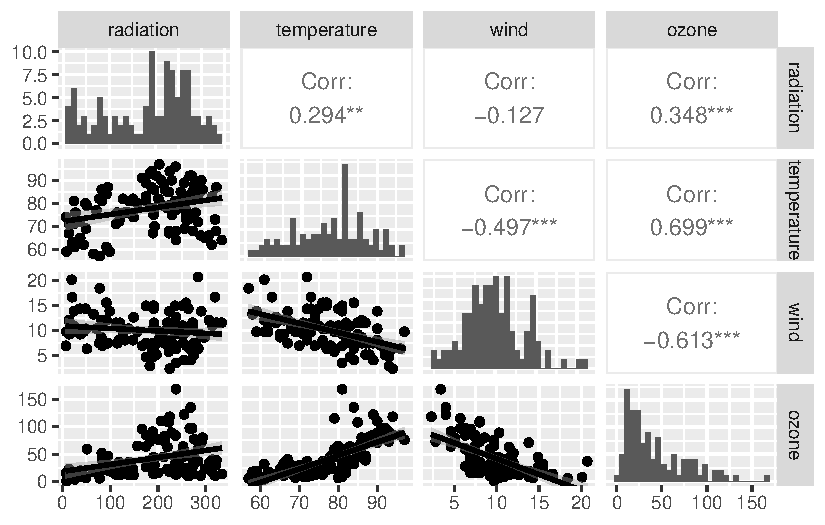
\includegraphics{StatsAssignment_files/figure-pdf/unnamed-chunk-6-1.pdf}

}

\end{figure}

Firstly, as it can be observed in the graph that ozone has a very
significant positive skewness and is possibly normally distributed. It
also noticeable from the ozone histogram that it resembles a normal
distribution with positive skewness.

We can also observe that ozone have a good correlation with temperature
with only a small amount of variance overall with the exception of a few
points between the 3rd quartile and the maximum, we can also see that
there is a a positive slope meaning that as temperature increases the
amount of ozone detected increases as well.

Furthermore, radiation has a correlation with a positive slope with
ozone so radiation has a positive effect on ozone. The variance is more
extreme between the 2nd quartile and maximum but maintaining a
relatively low variance between the minimum and the 2nd quartile.

Lastly, Wind's correlation with ozone has a negative slope, meaning that
has wind increases the less ozone is detected. Most of the variance
below the line of best fit, is between the first and third quartile
while the values that are more on the extreme, between the the minimum
and 1st quartile and the 3rd quartile and the maximum are almost all
above the line of best fit. The wind histogram also displays what looks
to be a normal distribution with close to zero skewness with some
irregularities near the 15 bin.

\#\#question 5 b)

\begin{Shaded}
\begin{Highlighting}[]
\NormalTok{model }\OtherTok{=} \FunctionTok{lm}\NormalTok{(ozone }\SpecialCharTok{\textasciitilde{}}\NormalTok{ radiation }\SpecialCharTok{+}\NormalTok{ temperature }\SpecialCharTok{+}\NormalTok{ wind, }\AttributeTok{data =}\NormalTok{ ozone)}

\FunctionTok{summary}\NormalTok{(model)}
\end{Highlighting}
\end{Shaded}

\begin{verbatim}

Call:
lm(formula = ozone ~ radiation + temperature + wind, data = ozone)

Residuals:
    Min      1Q  Median      3Q     Max 
-40.485 -14.210  -3.556  10.124  95.600 

Coefficients:
             Estimate Std. Error t value Pr(>|t|)    
(Intercept) -64.23208   23.04204  -2.788  0.00628 ** 
radiation     0.05980    0.02318   2.580  0.01124 *  
temperature   1.65121    0.25341   6.516 2.43e-09 ***
wind         -3.33760    0.65384  -5.105 1.45e-06 ***
---
Signif. codes:  0 '***' 0.001 '**' 0.01 '*' 0.05 '.' 0.1 ' ' 1

Residual standard error: 21.17 on 107 degrees of freedom
Multiple R-squared:  0.6062,    Adjusted R-squared:  0.5952 
F-statistic: 54.91 on 3 and 107 DF,  p-value: < 2.2e-16
\end{verbatim}

\begin{Shaded}
\begin{Highlighting}[]
\DocumentationTok{\#\# we can observe that the intercept so when \textbackslash{}t}

\DocumentationTok{\#\# residuals are the values of the differences between the line we made}
\DocumentationTok{\#\# and the observations}

\DocumentationTok{\#\# the coefficients are the point estimations intercept is the beta0}
\DocumentationTok{\#\# and the wt is the beta1}
\end{Highlighting}
\end{Shaded}

First thing we can observe is the confidence intervals of the 3
variables, both the temperature and wind have confidence intervals of
99,9\% as it can be see by the 3 stars next to their respective
p-values, radiation is in the 95\% confidence interval but is close to
the 99\% confidence interval.

From the estimates we can than wind is the variable with the biggest
impact per unit however when comparing it is also important to compare
using the minimum and maximum values so we can determine how much each
of the independent variables have been recorded to affect the ozone
readings so we will be using the minimum and maximum to determine the
maximum and minimum variance.

About the Coefficients, we can observe that radiation is the least
impactful of the 3 independent variables, the changes in ozone radiation
detected vary between {[}0.4186,19.9732{]} from the minimum and maximum
values, which compared to the {[}94.11897,160.16737{]} minimum and
maximum variance from the temperature readings which is by far the most
impactful variable or the {[}-7.67648,-66.752{]} variance from the
minimum and maximum values from the wind readings.

Are these findings consistent with your earlier descriptive plots? Also
include suitable residual plots, commenting as appropriate.

\hypertarget{the-intercept-value-is-impossible-so-lets-grpah-what-we-have-and-have-a-look}{%
\subsection{the intercept value is impossible so lets grpah what we have
and have a
look}\label{the-intercept-value-is-impossible-so-lets-grpah-what-we-have-and-have-a-look}}

Coefficients: Estimate Std. Error t value
Pr(\textgreater\textbar t\textbar)\\
(Intercept) -64.23208 23.04204 -2.788 0.00628 ** radiation 0.05980
0.02318 2.580 0.01124 *\\
temperature 1.65121 0.25341 6.516 2.43e-09 \textbf{\emph{wind -3.33760
0.65384 -5.105 1.45e-06}}

radiation temperature wind ozone\\
Min. : 7.0 Min. :57.00 Min. : 2.300 Min. : 1.0\\
1st Qu.:113.5 1st Qu.:71.00 1st Qu.: 7.400 1st Qu.: 18.0\\
Median :207.0 Median :79.00 Median : 9.700 Median : 31.0\\
Mean :184.8 Mean :77.79 Mean : 9.939 Mean : 42.1\\
3rd Qu.:255.5 3rd Qu.:84.50 3rd Qu.:11.500 3rd Qu.: 62.0\\
Max. :334.0 Max. :97.00 Max. :20.700 Max. :168.0

\(\beta0 = \beta1\)

\begin{Shaded}
\begin{Highlighting}[]
\FunctionTok{plot}\NormalTok{(model)}
\end{Highlighting}
\end{Shaded}

\begin{figure}[H]

{\centering 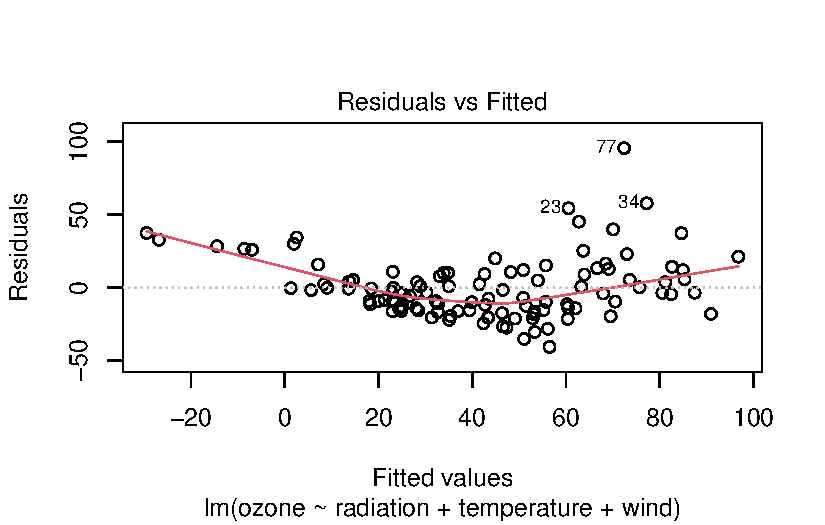
\includegraphics{StatsAssignment_files/figure-pdf/unnamed-chunk-8-1.pdf}

}

\end{figure}

\begin{figure}[H]

{\centering 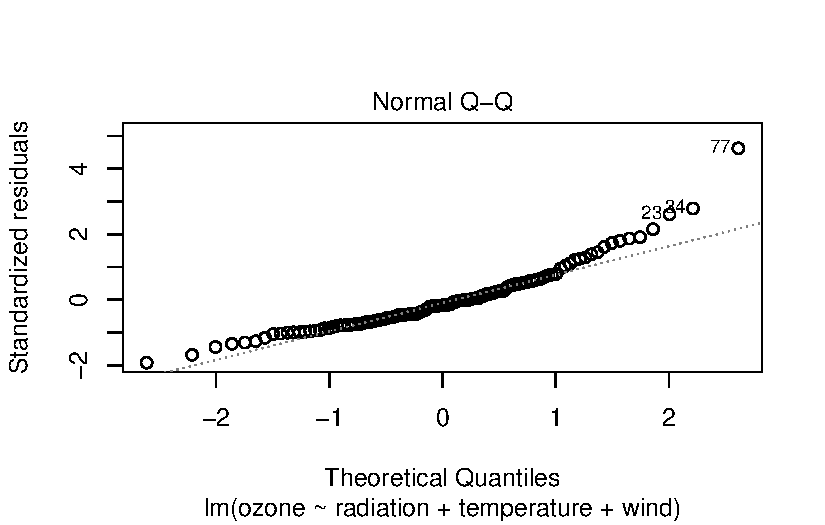
\includegraphics{StatsAssignment_files/figure-pdf/unnamed-chunk-8-2.pdf}

}

\end{figure}

\begin{figure}[H]

{\centering 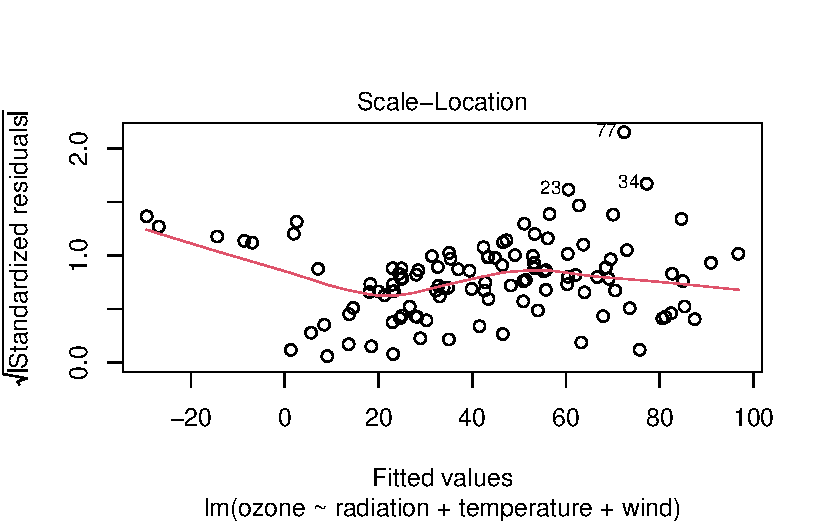
\includegraphics{StatsAssignment_files/figure-pdf/unnamed-chunk-8-3.pdf}

}

\end{figure}

\begin{figure}[H]

{\centering 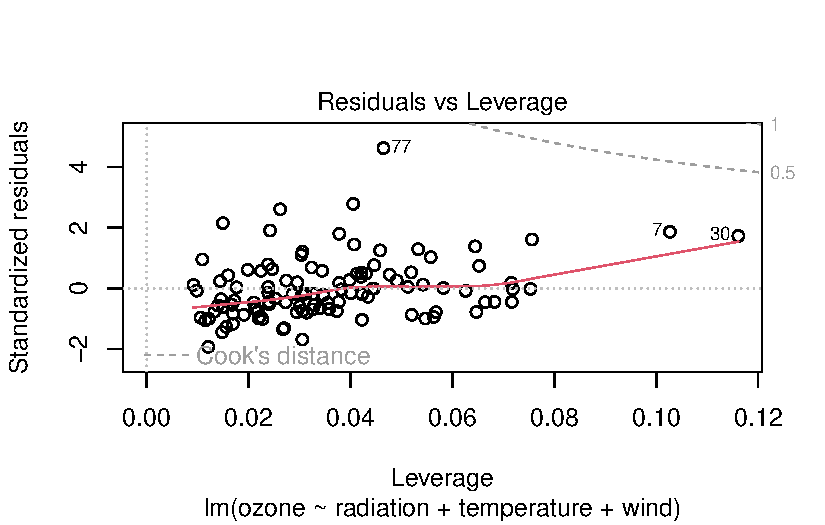
\includegraphics{StatsAssignment_files/figure-pdf/unnamed-chunk-8-4.pdf}

}

\end{figure}

\begin{Shaded}
\begin{Highlighting}[]
\DocumentationTok{\#\# a residual is the distance between our data points and our}
\DocumentationTok{\#\# regression line}
\end{Highlighting}
\end{Shaded}

As observed here on Residuals vs Fitted graph

\#\#question 5 c)

\begin{Shaded}
\begin{Highlighting}[]
\DocumentationTok{\#\# log(ozone) = β0+β1 log(radiation)+β2 log(temperature)+β3}
\DocumentationTok{\#\# log(wind)+εi where εi ∼ N (0, σ2) β0 = intercept}

\NormalTok{modelLogFriend }\OtherTok{=} \FunctionTok{lm}\NormalTok{(}\FunctionTok{log}\NormalTok{(ozone) }\SpecialCharTok{\textasciitilde{}} \FunctionTok{log}\NormalTok{(radiation) }\SpecialCharTok{+} \FunctionTok{log}\NormalTok{(temperature) }\SpecialCharTok{+} \FunctionTok{log}\NormalTok{(wind),}
    \AttributeTok{data =}\NormalTok{ ozone)}


\FunctionTok{summary}\NormalTok{(modelLogFriend)}
\end{Highlighting}
\end{Shaded}

\begin{verbatim}

Call:
lm(formula = log(ozone) ~ log(radiation) + log(temperature) + 
    log(wind), data = ozone)

Residuals:
     Min       1Q   Median       3Q      Max 
-1.63961 -0.30073 -0.00097  0.34414  1.11545 

Coefficients:
                  Estimate Std. Error t value Pr(>|t|)    
(Intercept)      -10.55570    2.08818  -5.055 1.79e-06 ***
log(radiation)     0.30500    0.05868   5.198 9.73e-07 ***
log(temperature)   3.20478    0.46019   6.964 2.79e-10 ***
log(wind)         -0.66305    0.13751  -4.822 4.74e-06 ***
---
Signif. codes:  0 '***' 0.001 '**' 0.01 '*' 0.05 '.' 0.1 ' ' 1

Residual standard error: 0.4907 on 107 degrees of freedom
Multiple R-squared:  0.6876,    Adjusted R-squared:  0.6788 
F-statistic: 78.49 on 3 and 107 DF,  p-value: < 2.2e-16
\end{verbatim}

\begin{Shaded}
\begin{Highlighting}[]
\FunctionTok{summary}\NormalTok{(model)}
\end{Highlighting}
\end{Shaded}

\begin{verbatim}

Call:
lm(formula = ozone ~ radiation + temperature + wind, data = ozone)

Residuals:
    Min      1Q  Median      3Q     Max 
-40.485 -14.210  -3.556  10.124  95.600 

Coefficients:
             Estimate Std. Error t value Pr(>|t|)    
(Intercept) -64.23208   23.04204  -2.788  0.00628 ** 
radiation     0.05980    0.02318   2.580  0.01124 *  
temperature   1.65121    0.25341   6.516 2.43e-09 ***
wind         -3.33760    0.65384  -5.105 1.45e-06 ***
---
Signif. codes:  0 '***' 0.001 '**' 0.01 '*' 0.05 '.' 0.1 ' ' 1

Residual standard error: 21.17 on 107 degrees of freedom
Multiple R-squared:  0.6062,    Adjusted R-squared:  0.5952 
F-statistic: 54.91 on 3 and 107 DF,  p-value: < 2.2e-16
\end{verbatim}



\end{document}
